\chapter{Augmenting Nanomolar High-Throughput Screening with Machine Learning for Lead Optimisation} \label{ch:testing}

Accurately determining the biological activity of a molecule requires compound synthesis and purification followed by preparation of a solution of known concentration to measure compound activity via an assay. While necessary for maximum accuracy, compound purification can be time-consuming and costly, bottlenecking the throughput of compound screening. This is a challenge particularly when exploring large and diverse sets of analogues for an intermediate hit or lead compound in order to derive its structure-activity relationship (SAR).

% TODO - not quite connected to the first paragraph
Recent work in developing nanomolar-scale high-throughput chemistry seeks to address this issue \cite{Santarilla2015MerckNanomolar, Perera2018PfizerNanomolar, Gehrtz2022nanomolar}. Adopting techniques from plate-based biological-assay screening, reacting one reagent with a different second reagent in each well of the plate, these approaches enable commonplace medicinal chemistry reactions (e.g., amide couplings and Suzuki reactions) to be conducted in a high-throughput manner with minimal starting material (<300 nmol). Utilising this method at the end of a synthesis route allows high-throughput generation of analogues for SAR exploration. In addition to higher throughput, nanomolar-scale chemistry also reduces costs by lowering solvent usage and conserving advance intermediates in the synthesis route. 

The drawback, however, is that it is rarely possible to perform purification for reactions conducted at the nanomole scale. The output of these reactions are therefore a mixture of chemical reactants, reagents, and products konwn as a crude reaction mixture. These reaction mixtures can still be assayed for measuring biological activity, but there will necessarily be additional noise as detected potency will be influenced by variations in reaction yield, or interference from the reactants. Nevertheless, nanomolar-scale synthesis combined with biochemical screening of crude reaction mixtures have been exploited for the discovery of potent inhibitors for several kinases \cite{Gesmundo2018nanosar, Gehrtz2022nanomolar}, illustrating the potential of this approach for accelerating hit-to-lead drug design.

A related approach for high-throughput synthesis are DNA-encoded libraries (DEL) \cite{GirondaMartinez2021DNALibrary}. By linking small molecule building blocks with DNA fragments before chemically enumerating the building blocks with one another, large and diverse combinatorial libraries can be generated. These libraries can be biochemically screened in crude as potent compounds which bind to the protein target can be identified by their DNA tags using high-throughput sequencing methods. There has been recent success in training ML models on DEL bioactivity screen for hit-finding \cite{McCloskey2020DNALibrary}, and the success of this approach suggest that applying ML to nanomolar screening data may also be possible.

In this chapter, we assess the utility of training ML models on bioacitvity data from nanomolar-scale high-throughput screening of crude reaction mixtures.

This is a novel assay technique delivering noisy data which has not been assessed for machine learning. Leave-one-out validation on the training data correctly identified false negatives, and a prospective virtual screen of EnamineREAL with the trained models returned top hits with similar potency and better pharmacokinetic properties.

% Such derivatization is preferably achieved toward the end of the synthesis route, to maximize the utility of a single intermediate. This approach can be readily scaled to plate-based format, where the starting material is reacted with a different second reagent in each well of the plate. Provided there is no interference from the other reagents in the reaction, this significantly increases the speed, reduces chemical waste and lowers the cost of initial SAR exploration. The plate-based format allows closer integration of chemical and biological experiments but also comes with the limitation that reactions conducted at the nanomole scale are rarely appropriate for purification.

% In collaboration with the London Lab at The Weizmann Institute of Science, we investigated whether we needed compound purification at all for training machine learning bioactivity models by using non-purified compound assays. Focusing on a particular scaffold synthesised with an peptide coupling as the final step, we added the acid and amine reactants directly in solution with the protein to obtain an assay reading from the crude reaction mixture. By skipping the purification step, this allowed us to quickly screen a library of 300 amines with the same acid in high-throughput which we used to train RF and GP models. 

% However, one overlooked area in this development cycle is ML applied as a filtering protocol for initial lead discovery, despite reports that ML methods often implicitly identify false positives and false negatives.6,7 Crude activity screening (assuming some level of introduction by Mihajlo is given previously) is a logical area to apply such techniques as noise and false hits/misses play a substantial role in obscuring valuable data. We hypothesized that combining two robust ML methodologies, Gaussian Processes (GPs) and Random Forests (RFs), could be used to identify hidden gems (false negatives) and overlooked molecules (low activity positives). Both GPs and RFs have been utilized in numerous chemoinformatics tasks, with several precedents in pharmaceutics development, making both ideal for predicting activity of novel compounds.8-12 Given the difference in approach to modeling for GPs and RFs, it was hypothesized that a combination of the two would lead to a highly robust framework; a compound predicted to have low activity from both a GP and a RF is likely to be inactive and likewise a compound with high predicted activity from both the GP and RF is likely potent.

\begin{figure}
    \centering
             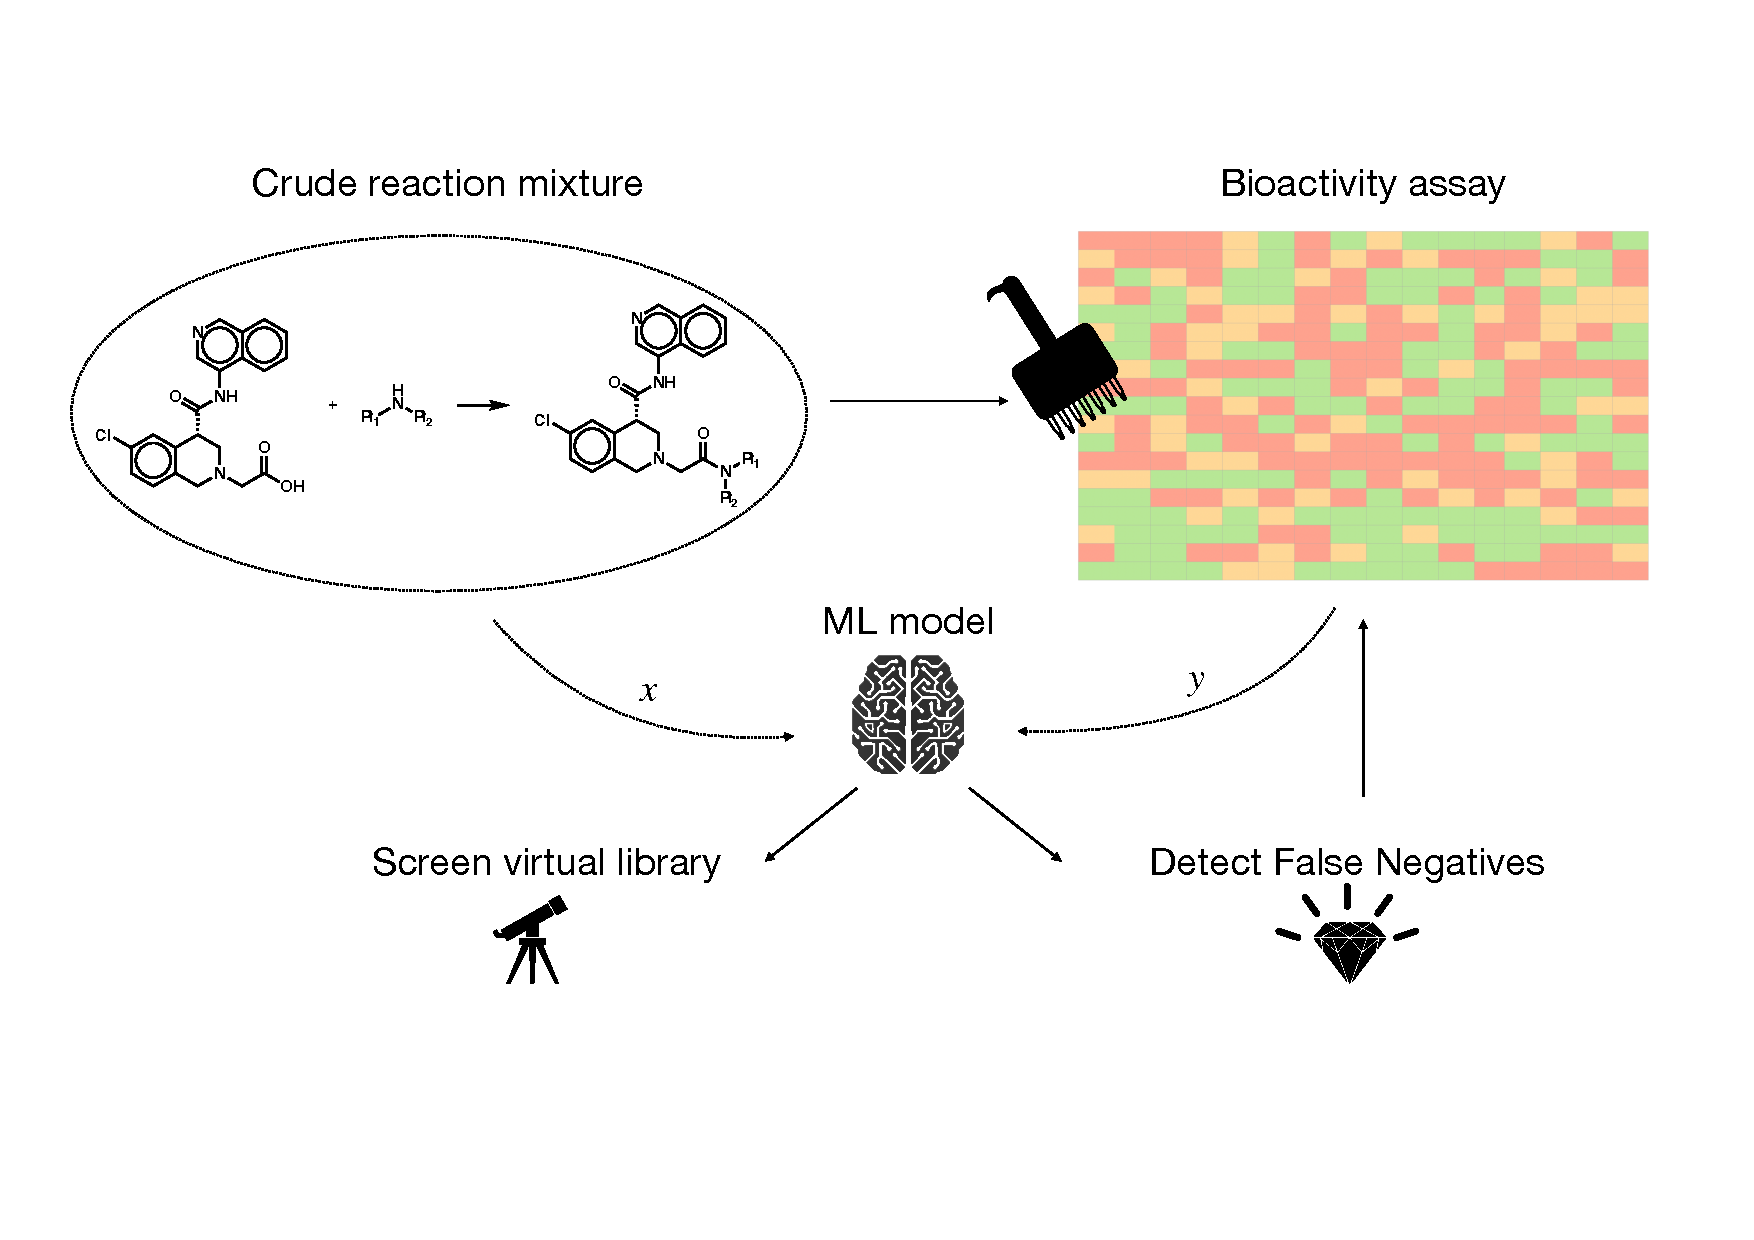
\includegraphics[width=\textwidth]{Chapters/Crude/Figs/schematic.pdf}
        \caption{Schematic of workflow.}
        \label{fig:schematic}
    \end{figure}

\section{Identifying False Negatives in Experimental Data}

\begin{figure}
    \centering
             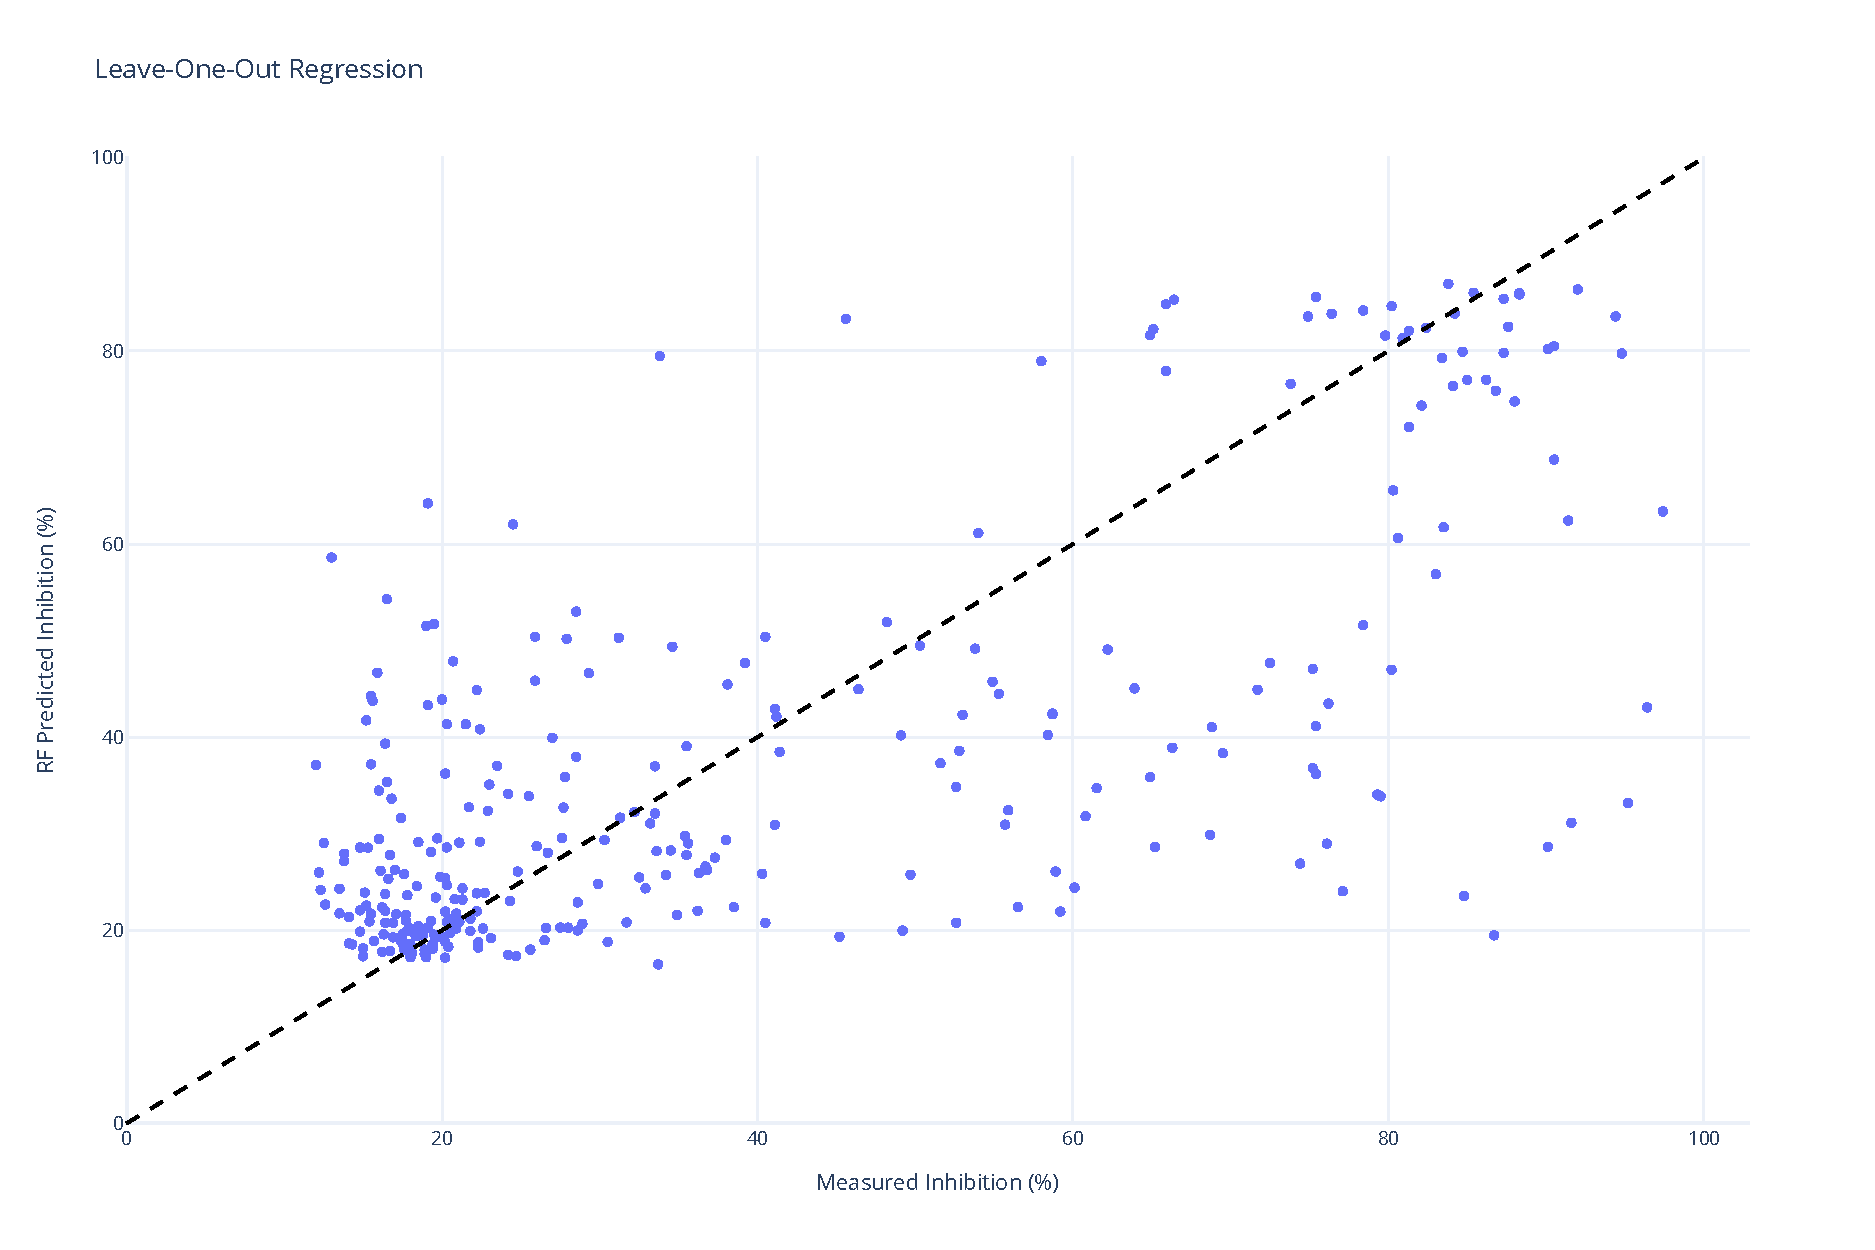
\includegraphics[width=\textwidth]{Chapters/Crude/Figs/rf.pdf}
        \caption{Leave one out regression.}
        \label{fig:leave-one-out}
    \end{figure}

Long discussion on the regressed performance. Disagreements between RF and GP model?

< Figure of the false negative >

Thus, we separately trained a GP and RF on the crude inhibition data, identifying 5 compounds which had predicted activity from both the GP and RF but no crude activity. We suspected that these were false negatives and re-synthesized, purified, and re-tested them with full dose-response curves to obtain IC50 inhibition values. This revealed that one of them was active with IC50 = 0.113\uM (ASAP-0000204). (needs a nice sentence to round it off).

TODO - broad discussion of model predictions, correlation with yield?
yields determind by integration of the UV spectra of each reaction.

Examples of two nanomole scale high throughput chemistry (HTC) campaigns to optimize the potency of intermediate binders. In one case we used the Chan-Lam reaction (Fig S7) and in another amide coupling (Fig S8). Direct biochemical screening of crude reactions identified candidates that were resynthesized and in both cases were able to improve the potency of the parent compound.

A complementary method for rapid SAR evaluation was the use of nanomole scale high-throughput chemistry(43, 44) (HTC), coupled with a 'direct to biology'(45-47) biochemical screening. The optimization of the amide coupling reaction to extend MAT-POS-4223bc15-21 (Figure 2D). The co-crystal structure of the parent compound (Fig S6) suggested vectors that could target the P4 pocket of Mpro. Optimization of the reaction conditions was performed for the starting building block with model amines (Figs S7-S8) and the optimal conditions were applied to HTC with a library of 300 amine building blocks. Yield estimation was performed and showed 151 of the library yielded >30\% of the desired product. Nevertheless, the crude mixtures were subjected to a biochemical assay against Mpro (Experimental details can be found in Appendix \ref{appendix:amide_coupling} \& \ref{appendix:mpro_assay}). 20 compounds were selected for resynthesis (Fig S9). In parallel to synthesis, the crude reaction mixtures were subjected to soaking and x-ray crystallography. The structures verified the extended compounds indeed adopt a similar binding mode to the parent, extending towards P3/P5 instead of the P4 pocket nevertheless forming new interactions with Mpro (Figure 2E). Upon resynthesis, several of the amide-coupling series were able to improve by up-to 300-fold on the parent acid-compound (up-to 3-fold on the corresponding methyl-amide) with the best inhibitor exhibiting an IC50 of 28nM.



\section{Scaffold Exploration via Virtual Screening}

Looking forward, we test the ability of the trained models to extrapolate to novel compounds by prospectively screening an external library of amides. 

We virtually enumerate primary and secondary amine building blocks from Enamine with the same carboxylic acid substructure from the crude activity screening. This results in a library of ~62,800 amides which were scored by the trained GP and RF models, and 

filtered for structural alerts and filtering out molecules with more than one chiral center to avoid complications in assessing potency.

we select the top 20 compounds with high predicted activity for both the GP and RF for synthesis and assaying to obtain IC50 values. 

Gratifyingly, the top 2 ML compounds showed promising average IC50 values of 0.0525\uM (ASAP-0000169) and 0.075\uM (ASAP-0000211), respectively. The top 2 most potent molecules based off of the crude inhibition values were compounds that, whilst active at IC50 = 0.034\uM (ASAP-0000221) and IC50 = 0.064\uM (ASAP-0000164), contained the toxic benzene-1,4-diamine motif that is generally avoided \cite{Kumar2011diallinine}. The top 2 compounds without the aforementioned motif derived from only crude inhibition values had similar pure compound IC50 values to our framework's identified compounds, 0.046\uM (ASAP-0000155) and 0.064\uM (ASAP-0000225), respectively. This result highlights ML's ability to identify promising yet overlooked scaffolds without compromising potency. 

\begin{figure}
    \centering
             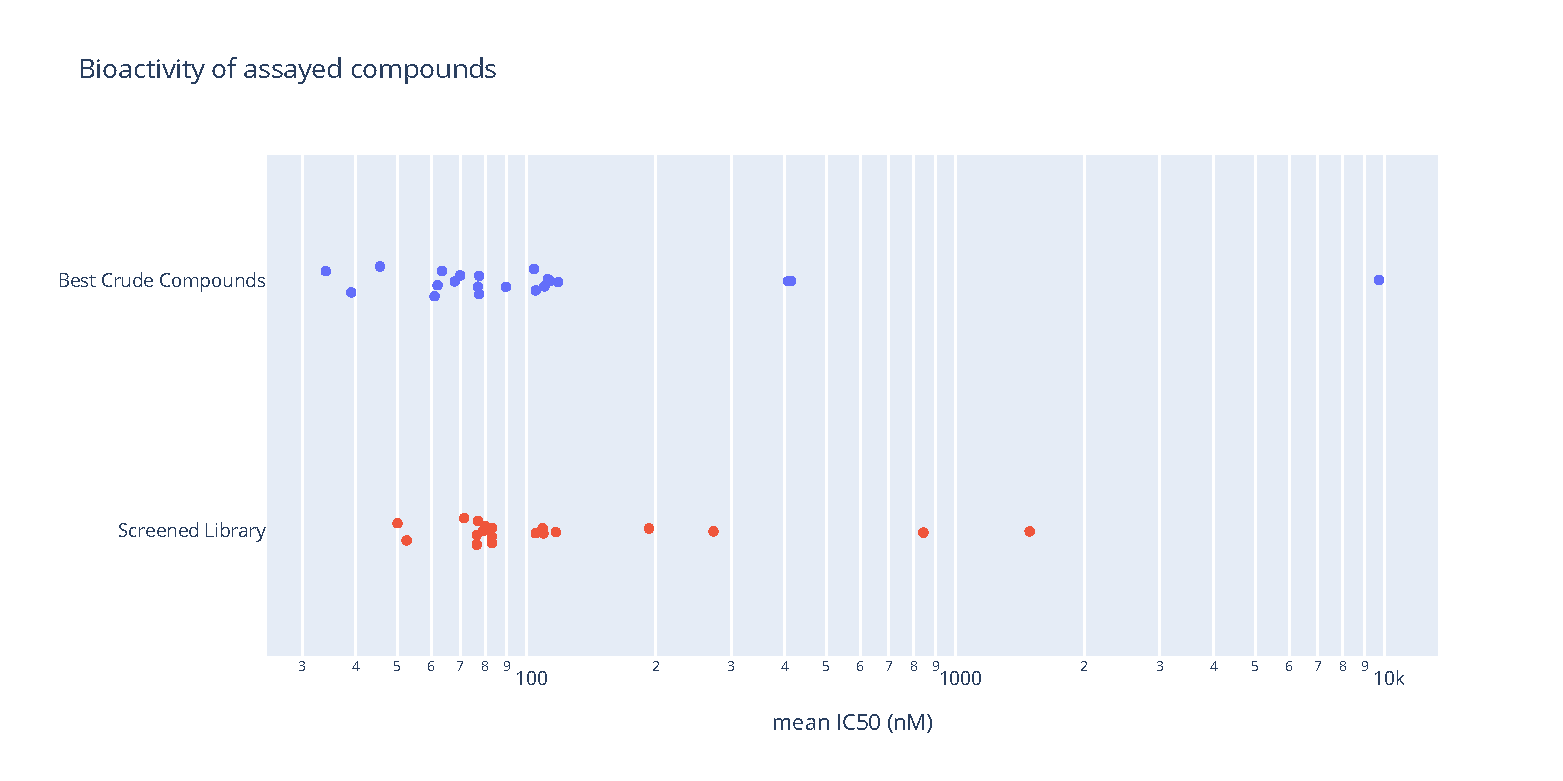
\includegraphics[width=\textwidth]{Chapters/Crude/Figs/strip_plot.pdf}
        \caption{Plot of mean IC50 values.}
        \label{fig:strip}
    \end{figure}

< Figure of the top 2 shown in panel B >

\section{Discussion}

Usefulness of training models with crude reaction mixtures. Not only is it useful for nanoSAR, it's very potent for generating data and screening libraries - ideal for setting up automated feedback loop and/or bayesian optimisation workflow.

Not limited to biochemical assays. Crude reaction mixtures for crystallographic fragment screening ~5 FTE days to set up and analyse, compared to an estimate of 15-20 FTE days for preparation, purification, characterisation and preparation of separate stock solution for each of the samples, additionally saving 35-50 litres of various solvents for workup and purification, and approximately sevenfold saving of reagents and solvents for synthetic operations. \cite{Baker2020FragementsFromCrude}